\chapter{STR solutions}
\begin{abox}
	Practice set 1 solutions
	\end{abox}
\begin{enumerate}
	\item Consider the decay process $\tau^{-} \rightarrow \pi^{-}+v_{\tau}$ in the rest frame of the $\tau^{-} .$The masses of the $\tau^{-}, \pi^{-}$and $v_{\tau}$ are $M_{\tau}, M_{\pi}$ and zero respectively.\\
	\textbf{A} The energy of $\pi^{-}$is
	{\exyear{NET JUNE 2011}}
\begin{tasks}(2)
	\task[\textbf{A.}] $\frac{\left(M_{\tau}^{2}-M_{\pi}^{2}\right) c^{2}}{2 M_{\tau}}$
	\task[\textbf{B.}]$\frac{\left(M_{\tau}^{2}+M_{\pi}^{2}\right) c^{2}}{2 M_{\tau}}$
	\task[\textbf{C.}]$\left(M_{\tau}-M_{\pi}\right) c^{2}$
	\task[\textbf{D.}]$\sqrt{M_{\tau} M_{\pi}} c^{2}$
\end{tasks}
\begin{answer}
	\begin{align*}
	\intertext { From conservation of energy }
	 M_{\tau} c^{2}&=E_{\pi}+E_{v} \text {. }\\
	E_{\pi}^{2}&=p^{2} c^{2}+M_{\pi}^{2} c^{4} \text { and } E_{v}^{2}=p^{2} c^{2} \text { since momentum of } \pi^{-} \text {and } v_{\tau} \text { is same. }\\
	M_{\tau} c^{2}&=E_{\pi}+E_{v}, M_{\pi}^{2} c^{4}=E_{\pi}^{2}-E_{v}^{2} \Rightarrow E_{\pi}-E_{v}=\frac{M_{\pi}^{2} c^{4}}{M_{\tau} c^{2}}\\
	E_{\pi}-E_{v}&=\frac{M_{\pi}^{2} c^{2}}{M_{\tau}} \text { and } E_{\pi}+E_{v}=M_{\tau} c^{2} \Rightarrow E_{\pi}=\frac{\left(M_{\tau}^{2}+M_{\pi}^{2}\right) c^{2}}{2 M_{\tau}}
	\end{align*}
	The correct option is \textbf{(b)}
\end{answer}
\textbf{B} The velocity of  $\pi^{-} \text {is }$
\begin{tasks}(1)
	\task[\textbf{A.}] $\frac{\left(M_{\tau}^{2}-M_{\pi}^{2}\right) c}{M_{\tau}^{2}+M_{\pi}^{2}}$
	\task[\textbf{B.}]$\frac{\left(M_{\tau}^{2}+M_{\pi}^{2}\right) c}{M_{\tau}^{2}-M_{\pi}^{2}}$ 
	\task[\textbf{C.}] $\frac{M_{\pi} c}{M_{\tau}}$
	\task[\textbf{D.}]$\frac{M_{\tau} c}{M_{\pi}}$
\end{tasks}
\begin{answer}
\begin{align*}
\text { Velocity of } \pi^{-} \quad E_{\pi}&=\frac{\left(M_{\tau}^{2}+M_{\pi}^{2}\right) c^{2}}{2 M_{\tau}}=\frac{M_{\pi} c^{2}}{\sqrt{1-\frac{v^{2}}{c^{2}}}} \Rightarrow\left(1-\frac{v^{2}}{c^{2}}\right)=\frac{4 M_{\pi}^{2} M_{\tau}^{2}}{\left(M_{\tau}^{2}+M_{\pi}^{2}\right)^{2}}\\
\Rightarrow \frac{v^{2}}{c^{2}}&=1-\frac{4 M_{\pi}^{2} M_{\tau}^{2}}{\left(M_{\tau}^{2}+M_{\pi}^{2}\right)^{2}}\\
\frac{v^{2}}{c^{2}}&=\frac{M_{\tau}^{4}+M_{\pi}^{4}+2 M_{\tau}^{2} M_{\pi}^{2}-4 M_{\pi}^{2} M_{\tau}^{2}}{\left(M_{\tau}^{2}+M_{\pi}^{2}\right)^{2}}\\
v&=\left(\frac{M_{\tau}^{2}-M_{\pi}^{2}}{M_{\tau}^{2}+M_{\pi}^{2}}\right) c
\end{align*}
The correct option is \textbf{(a)}	
\end{answer}

	\item A constant force $F$ is applied to a relativistic particle of rest mass $m$. If the particle starts from rest at $t=0$, its speed after a time $t$ is
	{\exyear{NET DEC 2011}}
\begin{tasks}(2)
	\task[\textbf{A.}] $\mathrm{Ft} / \mathrm{m}$
	\task[\textbf{B.}]$c \tanh \left(\frac{F t}{m c}\right)$
	\task[\textbf{C.}]$c\left(1-e^{-F t / m c}\right)$
	\task[\textbf{D.}]$\frac{F c t}{\sqrt{F^{2} t^{2}+m^{2} c^{2}}}$
\end{tasks}
\begin{answer}
	\begin{align*}
	\frac{d p}{d t}&=F \Rightarrow p=F t+c . \text { At } t=0, p=0 \text { so, } c=0\\
	p&=F t \Rightarrow \frac{m u}{\sqrt{1-\frac{u^{2}}{c^{2}}}}\\
	u&=\frac{\left(\frac{F}{m}\right) t}{\sqrt{1+\left(\frac{F t}{m c}\right)^{2}}}=\frac{F c t}{\sqrt{F^{2} t^{2}+m^{2} c^{2}}}\\
	\end{align*}
	The correct option is \textbf{(d)}
\end{answer}

	\item Two events separated by a (spatial) distance $9 \times 10^{9} \mathrm{~m}$, are simultaneous in one inertial frame. The time interval between these two events in a frame moving with a constant speed $0.8 c$ (where the speed of light $c=3 \times 10^{8} \mathrm{~m} / \mathrm{s}$ ) is
	{\exyear{NET JUNE 2012}}
\begin{tasks}(2)
	\task[\textbf{A.}] $60 \mathrm{~s}$
	\task[\textbf{B.}]$40 \mathrm{~s}$
	\task[\textbf{C.}]$20 s$
	\task[\textbf{D.}] $0 s$
\end{tasks}
\begin{answer}
	\begin{align*}
	x_{2}^{\prime}-x_{1}^{\prime}&=9 \times 10^{9} m \text { and } t_{2}^{\prime}-t_{1}^{\prime}=0 . \text { Then }\\
	t_{2}-t_{1}&=\left(\frac{t_{2}^{\prime}+\frac{v}{c^{2}} x_{2}^{\prime}}{\sqrt{1-\frac{v^{2}}{c^{2}}}}\right)-\left(\frac{t_{1}^{1}+\frac{v}{c^{2}} x_{1}^{\prime}}{\sqrt{1-\frac{v^{2}}{c^{2}}}}\right)\\
	t_{2}-t_{1}&=\frac{t_{2}^{\prime}-t_{1}^{\prime}}{\sqrt{1-\frac{v^{2}}{c^{2}}}}+\frac{v}{c^{2}} \frac{\left(x_{2}^{\prime}-x_{1}^{\prime}\right)}{\sqrt{1-\frac{v^{2}}{c^{2}}}}=\frac{v}{c^{2}} \frac{\left(x_{2}^{\prime}-x_{1}^{\prime}\right)}{\sqrt{1-\frac{v^{2}}{c^{2}}}}\\
	\text { Put } v&=0.8 c \quad \Rightarrow t_{2}-t_{1} \cong 40 \mathrm{sec}
	\end{align*}
	The correct option is \textbf{(b)}
\end{answer}

	\item What is proper time interval between the occurrence of two events if in one inertial frame events are separated by $7.5 \times 10^{8} \mathrm{~m}$ and occur $6.5 \mathrm{~s}$ apart?
	{\exyear{NET JUNE 2012}}
\begin{tasks}(2)
	\task[\textbf{A.}] $6.50 \mathrm{~s}$
	\task[\textbf{B.}]$6.00 \mathrm{~s}$
	\task[\textbf{C.}]$5.75 \mathrm{~s}$
	\task[\textbf{D.}]$5.00 \mathrm{~s}$
\end{tasks}
\begin{answer}
	\begin{align*}
	\text{Proper time interval}
	\Delta t=\sqrt{\left(\Delta t^{\prime}\right)^{2}-\frac{r^{2}}{c^{2}}}=\sqrt{(6.5)^{2}-\left(\frac{7.5}{3}\right)^{2}}=6 \text { sec. }
	\end{align*}
	The correct option is \textbf{(b)}
\end{answer}
	\item The muon has mass $105 \mathrm{MeV} / \mathrm{c}^{2}$ and mean life time $2.2 \mu \mathrm{s}$ in its rest frame. The mean distance traversed by a muon of energy $315 \mathrm{MeV}$ before decaying is approximately,
	{\exyear{NET DEC 2012}}

\begin{tasks}(2)
	\task[\textbf{A.}] $3 \times 10^{5} \mathrm{~km}$ 
	\task[\textbf{B.}]$2.2 \mathrm{~cm}$
	\task[\textbf{C.}]$6.6 \mu \mathrm{m}$
	\task[\textbf{D.}]$1.98 \mathrm{~km}$
\end{tasks}
\begin{answer}
	\begin{align*}
	\text { Since } E&=315 \mathrm{MeV} \text { and } m_{0}=105 \frac{\mathrm{MeV}}{c^{2}} \text {. }\\
	E=m c^{2} \Rightarrow E&=\frac{m_{0} c^{2}}{\sqrt{1-\frac{v^{2}}{c^{2}}}} \Rightarrow 315	\\
	315&=\frac{105}{\sqrt{1-\frac{v^{2}}{c^{2}}}} \Rightarrow v=0.94 c\\
	\text{Now}, t&=\frac{t_{0}}{\sqrt{1-\frac{v^{2}}{c^{2}}}}\\
	t_{0}&=2.2 \mu s \Rightarrow t=\frac{2.2 \times 10^{-6}}{\sqrt{1-\frac{8}{9}}} \Rightarrow t=6.6 \mu s\\
	\text { Now the distance traversed by muon is } v t&=0.94 c \times 6.6 \times 10^{-6}=1.86 \mathrm{~km} \text {. }
	\end{align*}
	The correct option is \textbf{(d)}
\end{answer}
	\item The area of a disc in its rest frame $S$ is equal to 1 (in some units). The disc will appear distorted to an observer $O$ moving with a speed $u$ with respect to $S$ along the plane of the disc. The area of the disc measured in the rest frame of the observer $O$ is $(c$ is the speed of light in vacuum)
	{\exyear{NET JUNE 2013}}
\begin{tasks}(2)
	\task[\textbf{A.}] $\left(1-\frac{u^{2}}{c^{2}}\right)^{1 / 2}$
	\task[\textbf{B.}]$\left(1-\frac{u^{2}}{c^{2}}\right)^{-1 / 2}$
	\task[\textbf{C.}]$\left(1-\frac{u^{2}}{c^{2}}\right)$
	\task[\textbf{D.}]$\left(1-\frac{u^{2}}{c^{2}}\right)^{-1}$
\end{tasks}
\begin{answer}
\begin{align*}
&\text { Area of disc from } \mathrm{S} \text { frame is } 1 \text { i.e. } \pi a^{2}=1 \text { or } \pi a \cdot a=1\\
&\text { Area of disc from } S^{\prime} \text { frame is } \pi a \cdot b=\pi a \cdot a \sqrt{1-\frac{u^{2}}{c^{2}}}=1 \cdot \sqrt{1-\frac{u^{2}}{c^{2}}}=\sqrt{1-\frac{u^{2}}{c^{2}}}\\
&\text { where } b=a \sqrt{1-\frac{u^{2}}{c^{2}}}
\end{align*}
The correct option is \textbf{(a)}	
\end{answer}

	\item The recently-discovered Higgs boson at the LHC experiment has a decay mode into a photon and a $Z$ boson. If the rest masses of the Higgs and $Z$ boson are $125 \mathrm{GeV} / \mathrm{c}^{2}$ and $90 \mathrm{GeV} / \mathrm{c}^{2}$ respectively, and the decaying Higgs particle is at rest, the energy of the photon will approximately be
	{\exyear{NET JUNE 2014}}

\begin{tasks}(2)
	\task[\textbf{A.}] $35 \sqrt{3} \mathrm{GeV}$
	\task[\textbf{B.}]$35 \mathrm{GeV}$
	\task[\textbf{C.}]$30 \mathrm{GeV}$
	\task[\textbf{D.}]$15 \mathrm{GeV}$
\end{tasks}
\begin{answer}
	\begin{align*}
	H_{B} &\rightarrow P_{H}+Z_{B}\\
	\intertext { From conservation of momentum }
	 0&=\vec{P}_{1}+\vec{P}_{2} \Rightarrow \vec{P}_{1}=-\vec{P}_{2} \Rightarrow\left|P_{1}\right|=\left|P_{2}\right|\\
	\text { Now } E_{H_{B}}&=E_{P_{H}}+E_{Z_{B}} \Rightarrow E_{P_{H}}+E_{Z_{B}}=M_{H_{B}} c^{2}\\
	E_{P_{H}}^{2}&=P_{1}^{2} c^{2}+0 \text { and } E_{Z_{B}}^{2}=P_{2}^{2} c^{2}+M_{Z_{B}}^{2} c^{4}\\
	&\Rightarrow\left(E_{Z_{B}}-E_{P_{H}}\right)\left(E_{Z_{B}}+E_{P_{H}}\right)=M_{Z_{B}}^{2} c^{4} \quad \because\left|P_{1}\right|=\left|P_{2}\right|\\
	&\Rightarrow E_{Z_{B}}-E_{P_{H}}=\frac{M_{Z_{B}}^{2} c^{4}}{M_{H_{B}} c^{2}}=\frac{M_{Z_{B}}^{2} c^{2}}{M_{H_{B}}} \quad \because E_{Z_{B}}+E_{P_{H}}=M_{H_{B}} c^{2}\\
	&\Rightarrow 2 E_{P_{H}}=M_{H_{B}} c^{2}-\frac{M_{z_{B}}^{2} c^{2}}{M_{H_{B}}} \Rightarrow E_{P_{H}}=\frac{\left(M_{H_{B}}^{2}-M_{z_{B}}^{2}\right) c^{2}}{M_{H_{B}}}\\
	&\Rightarrow E_{P_{H}}=\left(\frac{125 \times 125-90 \times 90}{2 \times 125}\right) \times \frac{c^{4}}{c^{4}}=30.1 \mathrm{GeV}
	\end{align*}
	The correct option is \textbf{(c)}
\end{answer}
	\item Consider three inertial frames of reference $A, B$ and $C$. the frame $B$ moves with a velocity $\frac{c}{2}$ with respect to $A$, and $C$ moves with a velocity $\frac{c}{10}$ with respect to $B$ in the same direction. The velocity of $C$ as measured in $A$ is
	{\exyear{NET JUNE 2015}}
\begin{tasks}(2)
	\task[\textbf{A.}] $\frac{3 c}{7}$
	\task[\textbf{B.}]$\frac{4 c}{7}$
	\task[\textbf{C.}]$\frac{c}{7}$
	\task[\textbf{D.}] $\frac{\sqrt{3} c}{7}$
\end{tasks}
\begin{answer}$\left. \right. $	\\
\begin{minipage}{0.5\textwidth}
		\begin{align*}
	v&=\frac{c}{2}, \quad u_{x}^{\prime}=\frac{c}{10}\\
	u_{x}&=\frac{u_{x}^{\prime}+v}{1+\frac{u^{\prime} v_{x}}{c^{2}}}=\frac{4 c}{7}
	\end{align*}
\end{minipage}
	\begin{minipage}{0.5\textwidth}
	\begin{figure}[H]
		\centering
		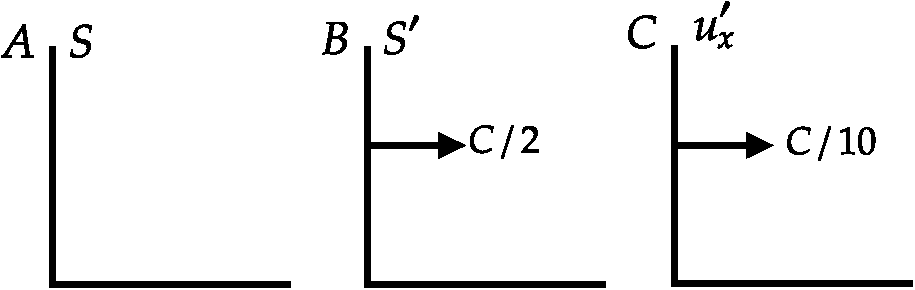
\includegraphics[height=3cm,width=5cm]{NET 1}
	\end{figure}
	\end{minipage}
The correct option is \textbf{(b)}
\end{answer}

	\item Consider a particle of mass $m$ moving with a speed $v$. If $T_{R}$ denotes the relativistic kinetic energy and $T_{N}$ its non-relativistic approximation, then the value of $\frac{\left(T_{R}-T_{N}\right)}{T_{R}}$ for $v=0.01 c$, is
	{\exyear{NET DEC 2015}}
\begin{tasks}(2)
	\task[\textbf{A.}] $1.25 \times 10^{-5}$
	\task[\textbf{B.}]$5.0 \times 10^{-5}$
	\task[\textbf{C.}]$7.5 \times 10^{-5}$
	\task[\textbf{D.}]$1.0 \times 10^{-4}$
\end{tasks}
\begin{answer}
	\begin{align*}
	T_{N}&=\frac{1}{2} m_{0} v^{2}, T_{R}=m c^{2}-m_{0} c^{2}=\frac{m_{0} c^{2}}{\sqrt{1-\frac{v^{2}}{c^{2}}}}-m_{0} c^{2} \quad(\because v=0.01 c)\\
	\text { Now, } \frac{\left(T_{R}-T_{N}\right)}{T_{R}}&=1-\frac{T_{N}}{T_{R}}=1-\frac{\frac{1}{2} m_{0} v^{2}}{\frac{m_{0} c^{2}}{\sqrt{1-\frac{v^{2}}{c^{2}}}}-m_{0} c^{2}}\\
	&=1-\frac{\frac{\frac{v^{2}}{2}}{c^{2}}}{\sqrt{1-\frac{v^{2}}{c^{2}}}-c^{2}}=1-\frac{\frac{(0.01)^{2}}{2}}{\frac{1}{\sqrt{1-(0.01)^{2}}}}-1\\
	\frac{T_{R}-T_{N}}{T_{R}}&=0.75
	\end{align*}
	None of the option is correct.
\end{answer}
	\item Let $(x, t)$ and $\left(x^{\prime}, t^{\prime}\right)$ be the coordinate systems used by the observers $O$ and $O^{\prime}$, respectively. Observer $O^{\prime}$ moves with a velocity $v=\beta c$ along their common positive $x$ axis. If $x_{+}=x+c t$ and $x_{-}=x-c t$ are the linear combinations of the coordinates, the Lorentz transformation relating $O$ and $O^{\prime}$ takes the form
	{\exyear{NET JUNE 2016}}
\begin{tasks}(2)
	\task[\textbf{A.}] $x_{+}^{\prime}=\frac{x_{-}-\beta x_{+}}{\sqrt{1-\beta^{2}}}$ and $x_{-}^{\prime}=\frac{x_{+}-\beta x_{-}}{\sqrt{1-\beta^{2}}}$
	\task[\textbf{B.}]$x_{+}^{\prime}=\sqrt{\frac{1+\beta}{1-\beta}} x_{+}$and $x_{-}^{\prime}=\sqrt{\frac{1-\beta}{1+\beta}} x_{-}$
	\task[\textbf{C.}]$x_{+}^{\prime}=\frac{x_{+}-\beta x_{-}}{\sqrt{1-\beta^{2}}}$ and $x_{-}^{\prime}=\frac{x_{-}-\beta x_{+}}{\sqrt{1-\beta^{2}}}$
	\task[\textbf{D.}]$x_{+}^{\prime}=\sqrt{\frac{1-\beta}{1+\beta}} x_{+}$and $x_{-}^{\prime}=\sqrt{\frac{1+\beta}{1-\beta}} x_{-}$
\end{tasks}
\begin{answer}
\begin{align*}
x_{+}^{\prime}&=x^{\prime}+c t^{\prime}\\
&=\frac{x-v t}{\sqrt{1-\frac{v^{2}}{c^{2}}}}+\frac{c\left(t-\frac{v x}{c^{2}}\right)}{\sqrt{1-\frac{v^{2}}{c^{2}}}}=\frac{x\left(1-\frac{v}{c}\right)}{\sqrt{1-\frac{v^{2}}{c^{2}}}}+\frac{c t\left(1-\frac{v}{c}\right)}{\sqrt{1-\frac{v^{2}}{c^{2}}}}\\
&=x \sqrt{\frac{1-\frac{v}{c}}{1+\frac{v}{c}}}+c t \sqrt{\frac{1-\frac{v}{c}}{1+\frac{v}{c}}}=\sqrt{\frac{1-\frac{v}{c}}{1+\frac{v}{c}}}(x+c t)\\
x_{+}^{\prime}&=\sqrt{\frac{1-\beta}{1+\beta}} x_{+}\\
x_{-}^{\prime}&=x^{\prime}-c t^{\prime}=\frac{x-v t}{\sqrt{1-\frac{v^{2}}{c^{2}}}}-\frac{c\left(t-\frac{v x}{c^{2}}\right)}{\sqrt{1-\frac{v^{2}}{c^{2}}}}=\frac{x\left(1+\frac{v}{c}\right)}{\sqrt{1-\frac{v^{2}}{c^{2}}}}-\frac{c t\left(1+\frac{v}{c}\right)}{\sqrt{1-\frac{v^{2}}{c^{2}}}}\\
x_{-}^{\prime}&=x \sqrt{\frac{1+\frac{v}{c}}{1-\frac{v}{c}}}-c t \sqrt{\frac{1+\frac{v}{c}}{1-\frac{v}{c}}} \Rightarrow x_{-}^{\prime}=\sqrt{\frac{1+\beta}{1-\beta}}(x-c t) \Rightarrow x_{-}^{\prime}=\sqrt{\frac{1+\beta}{1-\beta} x_{-}}
\end{align*}
The correct option is \textbf{(d)}	
\end{answer}

	\item For a particle of energy $E$ and momentum $p$ (in a frame $F$ ), the rapidity $y$ is defined as $y=\frac{1}{2} \ln \left(\frac{E+p_{3} c}{E-p_{3} c}\right) .$ In a frame $F^{\prime}$ moving with velocity $v=(0,0, \beta c)$ with respect to $F$, the rapidity $y^{\prime}$ will be
	{\exyear{NET JUNE 2016}}
\begin{tasks}(2)
	\task[\textbf{A.}] $y^{\prime}=y+\frac{1}{2} \ln \left(1-\beta^{2}\right)$
	\task[\textbf{B.}]$y^{\prime}=y-\frac{1}{2} \ln \left(\frac{1+\beta}{1-\beta}\right)$
	\task[\textbf{C.}]$y^{\prime}=y+\ln \left(\frac{1+\beta}{1-\beta}\right)$
	\task[\textbf{D.}]$y^{\prime}=y+2 \ln \left(\frac{1+\beta}{1-\beta}\right)$
\end{tasks}
\begin{answer}
\begin{align*}
y&=\frac{1}{2} \ln \left(\frac{E+p_{3} c}{E-p_{3} c}\right)\\
\text { Then } y^{\prime}&=\frac{1}{2} \ln \left(\frac{E^{\prime}+p_{3}^{\prime} c}{E^{\prime}-p_{3}^{\prime} c}\right)\\
\text { Where } p_{3}^{\prime}&=\gamma\left(p_{3}-v\left(\frac{E}{c^{2}}\right)\right) \quad E^{\prime}=\gamma\left(E-v p_{3}\right)\\
\text { Put the value of } p_{3}^{\prime} \text { and } E^{\prime} \text { one will get } y^{\prime}&=\frac{1}{2} \ln \left(\frac{\left(E+p_{3} c\right)-\frac{v}{c}\left(E+p_{3} c\right)}{\left(E-p_{3} c\right)+\frac{v}{c}\left(E-p_{3} c\right)}\right)\\
\frac{1}{2} \ln \left(\frac{\left(E+p_{3} c\right)(1-\beta)}{\left(E-p_{3} c\right)(1+\beta)}\right) &\Rightarrow \frac{1}{2} \ln \left(\frac{\left(E+p_{3} c\right)}{\left(E-p_{3} c\right)}\right)+\frac{1}{2} \ln \left(\frac{1-\beta}{1+\beta}\right)\\
y+\frac{1}{2} \ln \left(\frac{1-\beta}{1+\beta}\right)& \Rightarrow y-\frac{1}{2} \ln \left(\frac{1+\beta}{1-\beta}\right)
\end{align*}
The correct option is \textbf{(b)}	
\end{answer}
	\item A relativistic particle moves with a constant velocity $v$ with respect to the laboratory frame. In time $\tau$, measured in the rest frame of the particle, the distance that it travels in the laboratory frame is
	{\exyear{NET DEC 2016}}
\begin{tasks}(2)
	\task[\textbf{A.}] $v \tau$
	\task[\textbf{B.}]$\frac{c \tau}{\sqrt{1-\frac{v^{2}}{c^{2}}}}$
	\task[\textbf{C.}]$v \tau \sqrt{1-\frac{v^{2}}{c^{2}}}$
	\task[\textbf{D.}]$\frac{v \tau}{\sqrt{1-\frac{v^{2}}{c^{2}}}}$
\end{tasks}
\begin{answer}$\left. \right. $\\
	\begin{minipage}{0.5\textwidth}
	\begin{align*}
	\text { From Particle } x_{1}^{\prime}&=0 x_{2}^{\prime}=0\\
	t_{\text {initial }}&=t_{1}^{\prime} \quad t_{\text {final }}=t_{2}^{\prime}\\
	x_{1}&=\frac{x_{1}^{\prime}+v t_{1}^{\prime}}{\sqrt{1-v^{2} / c^{2}}}, x_{2}=\frac{x_{2}^{\prime}+v t_{2}^{\prime}}{\sqrt{1-v^{2} / c^{2}}}\\
	x_{2}-x_{1}&=\frac{x_{2}^{\prime}-x_{1}^{\prime}}{\sqrt{1-v^{2} / c^{2}}}+\frac{v\left(t_{2}^{\prime}-t_{1}^{\prime}\right)}{\sqrt{1-v^{2} / c^{2}}}\\
	\Delta x&=\frac{v\left(t_{2}^{\prime}-t_{1}^{\prime}\right)}{\sqrt{1-v^{2} / c^{2}}}=\frac{v \tau}{\sqrt{1-v^{2} / c^{2}}}
	\end{align*}	
	\end{minipage}
\begin{minipage}{0.5\textwidth}
	\begin{figure}[H]
		\centering
		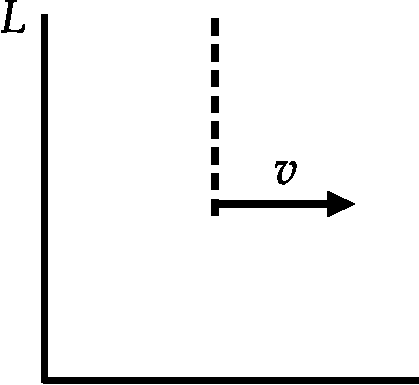
\includegraphics[height=3cm,width=5cm]{problem 2}
	\end{figure}
\end{minipage}
The correct option is \textbf{(d)}
\end{answer}
	\item Consider a radioactive nucleus that is travelling at a speed $\frac{c}{2}$ with respect to the lab frame. It emits $\gamma$-rays of frequency $v_{0}$ in its rest frame. There is a stationary detector, (which is not on the path of the nucleus) in the lab. If a $\gamma$-ray photon is emitted when the nucleus is closest to the detector, its observed frequency at the detector is
	{\exyear{NET DEC 2016}}
\begin{tasks}(2)
	\task[\textbf{A.}] $\frac{\sqrt{3}}{2} v_{0}$
	\task[\textbf{B.}]$\frac{1}{\sqrt{3}} v_{0}$
	\task[\textbf{C.}]$\frac{1}{\sqrt{2}} v_{0}$
	\task[\textbf{D.}]$\sqrt{\frac{2}{3}} v_{0}$
\end{tasks}
\begin{answer}
	\begin{align*}
	v&=v_{0} \sqrt{1-\frac{v^{2}}{c^{2}}} \quad \text { (If detector is not in the path at nucleus) }\\
	v&=v_{0} \sqrt{1-\frac{1}{4}}=v_{0} \frac{\sqrt{3}}{2}
	\end{align*}
	The correct option is \textbf{(a)}
\end{answer}
	\item An inertial observer sees two events $E_{1}$ and $E_{2}$ happening at the same location but $6 \mu s$ apart in time. Another observer moving with a constant velocity $v$ (with respect to the first one) sees the same events to be $9 \mu s$ apart. The spatial distance between the events, as measured by the second observer, is approximately
	{\exyear{NET JUNE 2017}}

\begin{tasks}(2)
	\task[\textbf{A.}] $300 m$
	\task[\textbf{B.}]$1000 m$
	\task[\textbf{C.}]$2000 m$
	\task[\textbf{D.}]$2700 m$
\end{tasks}
\begin{answer}
\begin{align*}
	x_{2}^{1}-x_{1}^{1}&=0, t_{2}^{1}-t_{1}^{1}=6 \times 10^{-6}, t_{2}-t_{1}=9 \times 10^{-6}, x_{2}-x_{1}=?\\
t_{2}-t_{2}&=9 \times 10^{-6}\\
\left(\frac{t_{2}^{1}+\frac{v}{c^{2}} x_{2}^{1}}{\sqrt{1-v^{2} / c^{2}}}\right)-\frac{\left(t_{1}^{\prime}+\frac{v}{c^{2}} x_{1}^{\prime}\right)}{\sqrt{1-v^{2} / c^{2}}}&=9 \times 10^{-6}\\
\frac{t_{2}^{\prime}-t_{1}^{\prime}}{\sqrt{1-v^{2} / c^{2}}}&=9 \times 10^{-6} \Rightarrow \frac{6 \times 10^{-6}}{\sqrt{1-v^{2} / c^{2}}}=9 \times 10^{-6}\\
v&=\sqrt{\frac{5}{9}} c \Rightarrow \sqrt{1-\frac{v^{2}}{c^{2}}}=2 / 3\\
\left(x_{2}-x_{1}\right)&=\left(\frac{x_{2}^{\prime}+v t_{2}^{\prime}}{\sqrt{1-v^{2} / c^{2}}}\right)-\left(\frac{x_{1}^{\prime}+v t_{1}^{\prime}}{\sqrt{1-v^{2} / c^{2}}}\right)\\
\frac{v}{\sqrt{1-v^{2} / c^{2}}}\left(t_{2}^{\prime}-t_{1}^{\prime}\right)\\
\left(x_{2}-x_{1}\right)&=\frac{\sqrt{5}}{3} c \times \frac{9}{6} \times\left(6 \times 10^{-6}\right)=\frac{\sqrt{5}}{3} \times 3 \times 10^{8} \times \frac{9}{6} \times 6 \times 10^{-6}\\
&=9 \times \sqrt{5} \times 10^{2}=20.12 \times 10^{2} \simeq 2000 m
\end{align*}
The correct option is \textbf{(c)}
\end{answer}
	\item A light signal travels from a point $A$ to a point $B$, both within a glass slab that is moving with uniform velocity (in the same direction as the light) with speed $0.3 c$ with respect to an external observer. If the refractive index of the slab is $1.5$, then the observer will measure the speed of the signal as
	{\exyear{NET DEC 2017}}
\begin{tasks}(2)
	\task[\textbf{A.}] $0.67 c$
	\task[\textbf{B.}]$0.81 c$
	\task[\textbf{C.}]$0.97 c$
	\task[\textbf{D.}] $c$
\end{tasks}
\begin{answer}$\left. \right. $\\
	\begin{minipage}{0.5\textwidth}
\begin{align*}
v&=0.3 c\\
u_{x}^{\prime}&=\frac{c}{n} n=1.5\\
u_{x}&=\frac{u_{x}^{\prime}+v}{1+\frac{u_{x}^{\prime} v}{c^{2}}}=\frac{0.3 c+\frac{c}{n}}{1+\frac{c}{n} \cdot \frac{0.3 c}{c^{2}}}\\
u_{x}&=0.81 c
\end{align*}
	\end{minipage}
\begin{minipage}{0.5\textwidth}
\begin{figure}[H]
	\centering
	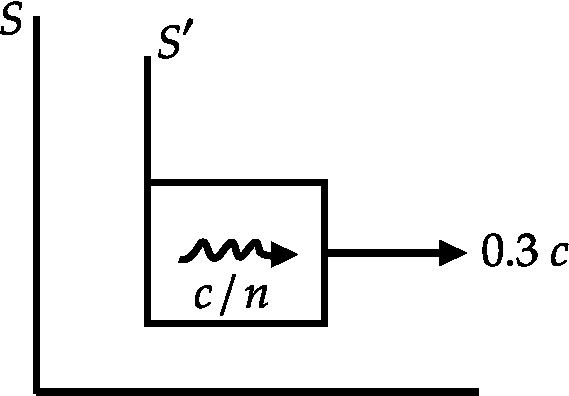
\includegraphics[height=3cm,width=5cm]{problem 4}
\end{figure}
\end{minipage}
The correct option is \textbf{(b)}
\end{answer}
	\item Two particles $A$ and $B$ move with relativistic velocities of equal magnitude $v$, but in opposite directions, along the $x$-axis of an inertial frame of reference. The magnitude of the velocity of $A$, as seen from the rest frame of $B$, is
	{\exyear{NET JUNE 2018}}

\begin{tasks}(2)
	\task[\textbf{A.}] $\frac{2 v}{\left(1-\frac{v^{2}}{c^{2}}\right)}$ 
	\task[\textbf{B.}]$\frac{2 v}{\left(1+\frac{v^{2}}{c^{2}}\right)}$
	\task[\textbf{C.}] $2 v \sqrt{\frac{c-v}{c+v}}$ 
	\task[\textbf{D.}]$\frac{2 v}{\sqrt{1-\frac{v^{2}}{c^{2}}}}$
\end{tasks}
\begin{answer}
	\begin{align*}
	u_{x}^{\prime}&=v \quad V=v\\
	u_{x}&=\frac{u_{x}^{\prime}+V}{1+\frac{u_{x} V}{c^{2}}}\\
	u_{x}&=\frac{v+v}{1+\frac{v^{2}}{c^{2}}}=\frac{2 v}{1+\frac{v^{2}}{c^{2}}}
	\end{align*}
	The correct option is \textbf{(b)}
\end{answer}

	\item The energy of a free relativistic particle is $E=\sqrt{|\vec{p}|^{2} c^{2}+m^{2} c^{4}}$, where $m$ is its rest mass, $\vec{p}$ is its momentum and $c$ is the speed of light in vacuum. The ratio $v_{g} / v_{p}$ of the group velocity $v_{g}$ of a quantum mechanical wave packet (describing this particle) to the phase velocity $v_{p}$ is
	{\exyear{NET JUNE 2018}}
\begin{tasks}(2)
	\task[\textbf{A.}] $|\vec{p}| c / E$
	\task[\textbf{B.}]$|\vec{p}| m c^{3} / E^{2}$
	\task[\textbf{C.}] $|\vec{p}|^{2} c^{3} / E^{2}$
	\task[\textbf{D.}]$|\vec{p}| c / 2 E$
\end{tasks}
	\begin{answer}
		\begin{align*}
		E^{2}&=p^{2} c^{2}+m^{2} c^{4} \text { and } v_{g}=\frac{d E}{d p}, v_{p}=\frac{E}{p}\\
		2 E \frac{d E}{d p}&=2 p c^{2} \Rightarrow \frac{E}{p} \frac{d E}{d p}=c^{2}\\
		\frac{v_{g}}{v_{p}}&=\frac{c^{2}}{v_{p}^{2}} \quad \frac{v_{g}}{v_{p}}=\frac{c^{3} p^{2}}{E^{2}}
		\end{align*}
		The correct option is \textbf{(c)}
\end{answer}
	\item An inertial frame $K^{\prime}$ moves with a constant speed $v$ with respect to another inertial frame $K$ along their common $x$ - direction. Let $(x, c t)$ and $\left(x^{\prime}, c t^{\prime}\right)$ denote the spacetime coordinates in the frames $K$ and $K^{\prime}$, respectively. Which of the following spacetime diagrams correctly describes the $t^{\prime}$ - axis $\left(x^{\prime}=0\right.$ line $)$ and the $x^{\prime}$ - axis $\left(t^{\prime}=0\right.$ line $)$ in the $x$-ct plane? (In the following figures $\tan \phi=v / c$ )
{	\exyear{NET JUNE 2018}}
\begin{tasks}(2)
	\task[\textbf{A.}]\begin{figure}[H]
		\centering
		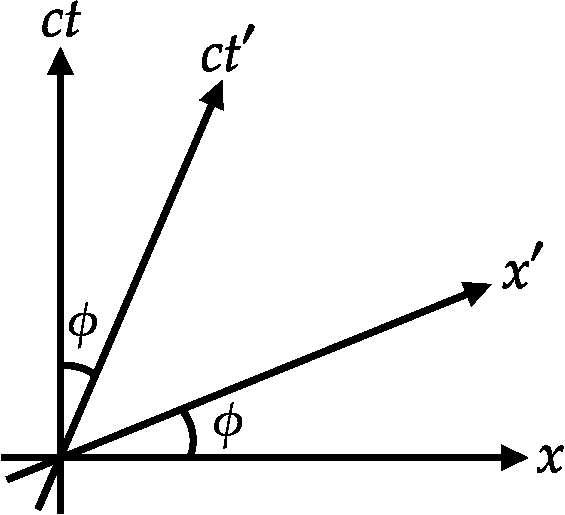
\includegraphics[height=4cm,width=5cm]{PROBLEM 5}
	\end{figure}
	\task[\textbf{B.}]\begin{figure}[H]
		\centering
		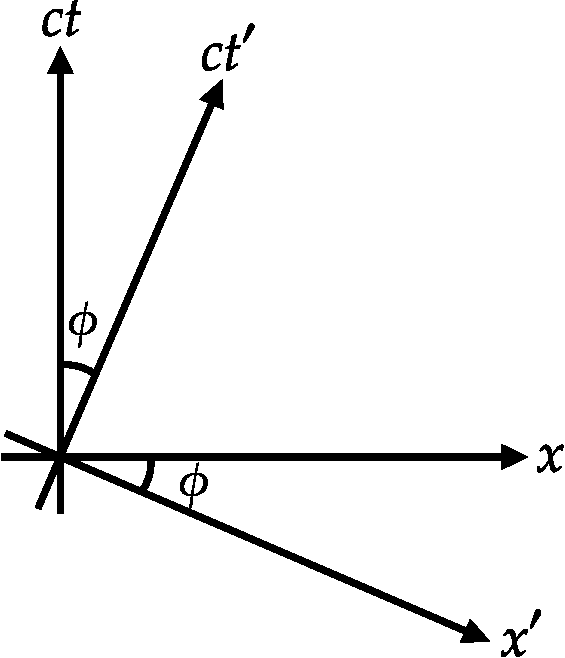
\includegraphics[height=4cm,width=5cm]{PROBLEM 6}
	\end{figure}
	\task[\textbf{C.}]\begin{figure}[H]
		\centering
		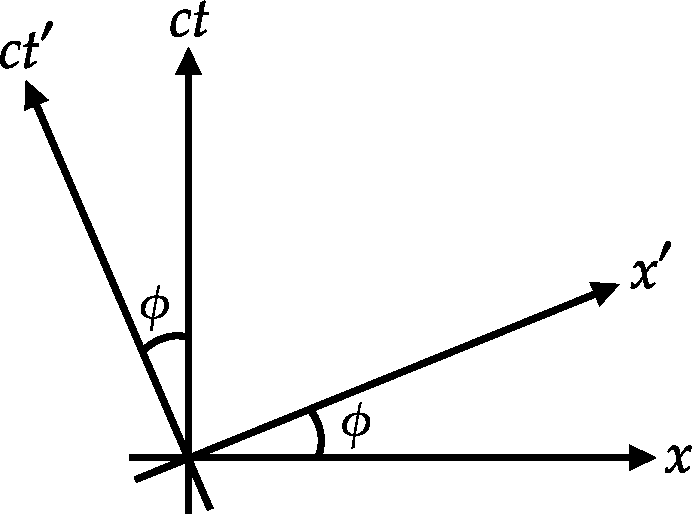
\includegraphics[height=4cm,width=5cm]{PROBLEM 7}
	\end{figure}
	\task[\textbf{D.}]\begin{figure}[H]
		\centering
		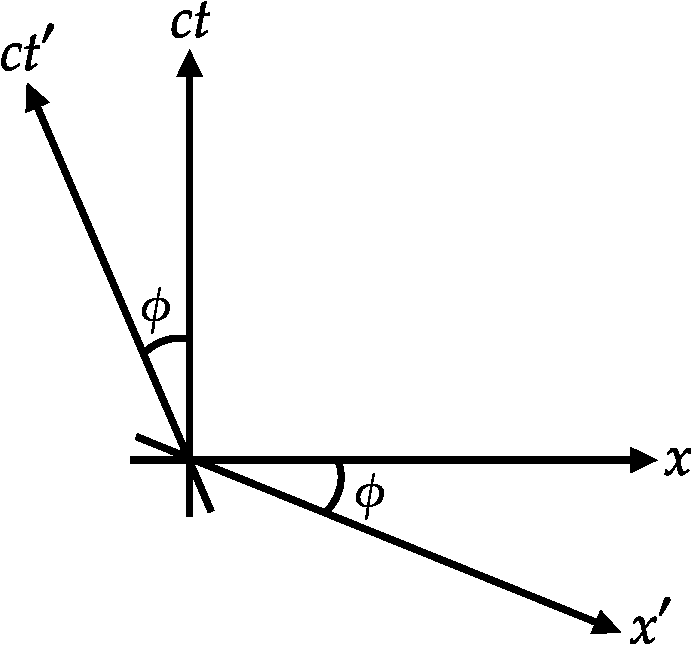
\includegraphics[height=4cm,width=5cm]{PROBLEM8}
	\end{figure}
\end{tasks}
\begin{answer}
$	\left(\begin{array}{c}
		c t^{\prime} \\
		x^{\prime} \\
		y^{\prime} \\
		z^{\prime}
	\end{array}\right)=\left(\begin{array}{cccc}
		\cosh \phi & -\sinh \phi & 0 & 0 \\
		-\sinh \phi & \cos \phi & 0 & 0 \\
		0 & 0 & 1 & 0 \\
		0 & 0 & 0 & 1
	\end{array}\right)\left(\begin{array}{l}
		c t \\
		x \\
		y \\
		z
	\end{array}\right)$\\
	$\text { Where } v=\cosh \phi, \beta v=\sinh \phi \beta=\tanh \phi$\\
	The correct option is \textbf{(a)}
\end{answer}

	\item A relativistic particle of mass $m$ and charge $e$ is moving in a uniform electric field of strength $\varepsilon$. Starting from rest at $t=0$, how much time will it take to reach the speed $\frac{c}{2}$ ?
	{\exyear{NET DEC 2018}}
\begin{tasks}(2)
	\task[\textbf{A.}] $\frac{1}{\sqrt{3}} \frac{m c}{e \varepsilon}$
	\task[\textbf{B.}]$\frac{m c}{e \varepsilon}$
	\task[\textbf{C.}]$\sqrt{2} \frac{m c}{e \varepsilon}$
	\task[\textbf{D.}]$\sqrt{\frac{3}{2}} \frac{m c}{e \varepsilon}$
\end{tasks}
\begin{answer}
\begin{align*}
\frac{d p}{d t}&=e \varepsilon\\
p&=e \varepsilon t+c\\
\text { At } t&=0, p=0, c=0\\
\frac{m v}{\sqrt{1-\frac{v^{2}}{c^{2}}}}&=e \varepsilon t\\
t&=\frac{m}{e \varepsilon} \frac{v}{\sqrt{1-\frac{v^{2}}{c^{2}}}}\\
\text { Put } v&=\frac{c}{2}, \quad t=\frac{m}{e \varepsilon} \frac{c / 2}{\sqrt{1-\frac{1}{4}}}=\frac{m c}{\sqrt{3} e \varepsilon}\\
t&=\frac{m c}{\sqrt{3} e E}
\end{align*}
The correct option is \textbf{(a)}	
\end{answer}
\end{enumerate}
\newpage
\begin{abox}
	Practice set 2 solutions
	\end{abox}
\begin{enumerate}

	\item For the set of all Lorentz transformations with velocities along the $x$-axis consider the two statements given below:
	P: If $L$ is a Lorentz transformation, then, $L^{-1}$ is also a Lorentz transformation.
	Q: If $L_{1}$ and $L_{2}$ are Lorentz transformations, then $L_{1} L_{2}$ is necessarily a Lorentz transformation.
	Choose the correct option
	{\exyear{GATE 2010}}

\begin{tasks}(2)
	\task[\textbf{A.}] $P$ is true and $Q$ is false
	\task[\textbf{B.}]Both $P$ and $Q$ are true
	\task[\textbf{C.}]Both $P$ and $Q$ are false
	\task[\textbf{D.}]$P$ is false and $Q$ is true
\end{tasks}
\begin{answer}
The correct option is \textbf{(b)}
\end{answer}
	\item A $\pi^{0}$ meson at rest decays into two photons, which moves along the $x$-axis. They are both detected simultaneously after a time, $t=10 \mathrm{~s} .$ In an inertial frame moving with a velocity $v=0.6 c$ in the direction of one of the photons, the time interval between the two detections is
	{\exyear{GATE 2010}}

\begin{tasks}(2)
	\task[\textbf{A.}] $15 c$
	\task[\textbf{B.}]$0 \mathrm{~s}$
	\task[\textbf{C.}] $10 \mathrm{~s}$
	\task[\textbf{D.}]$20 s$
\end{tasks}
\begin{answer}
\begin{align*}
t_{1}&=t_{0} \sqrt{\frac{1+\frac{v}{c}}{1-\frac{v}{c}}}=10 \sqrt{\frac{1+0.6}{1-0.6}}=10 \times 2=20 \mathrm{sec}\\
t_{2}&=t_{0} \sqrt{\frac{1-\frac{v}{c}}{1+\frac{v}{c}}}=10 \sqrt{\frac{1-0.6}{1+0.6}}=10 \times \frac{1}{2}=5 \mathrm{sec}\\
\mathrm{t}_{1}-\mathrm{t}_{2}&=15 \mathrm{sec}
\end{align*}	
The correct option is \textbf{(a)}
\end{answer}
	\item Two particles each of rest mass $m$ collide head-on and stick together. Before collision, the speed of each mass was $0.6$ times the speed of light in free space. The mass of the final entity is
{	\exyear{GATE 2011}}
\begin{tasks}(2)
	\task[\textbf{A.}] $5 m / 4$
	\task[\textbf{B.}]$2 m$
	\task[\textbf{C.}]$5 \mathrm{~m} / 2$
	\task[\textbf{D.}]$25 \mathrm{~m} / \mathrm{s}$
\end{tasks}
\begin{answer}
From conservation of energy\\
$$
\frac{m c^{2}}{\sqrt{1-\frac{v^{2}}{c^{2}}}}+\frac{m c^{2}}{\sqrt{1-\frac{v^{2}}{c^{2}}}}=m_{1} c^{2} \Rightarrow \frac{2 m c^{2}}{\sqrt{1-\frac{v^{2}}{c^{2}}}}=m_{1} c^{2}
$$
Since $v=0.6 c \Rightarrow m_{1}=5 \mathrm{~m} / 2$	\\
The correct option is \textbf{(c)}
\end{answer}
	\item A rod of proper length $l_{0}$ oriented parallel to the $x$-axis moves with speed $2 c / 3$ along the $x$-axis in the $S$-frame, where $c$ is the speed of light in free space. The observer is also moving along the $x$-axis with speed $c / 2$ with respect to the $S$-frame. The length of the rod as measured by the observer is
	{\exyear{GATE 2012}}
\begin{tasks}(2)
	\task[\textbf{A.}] $0.35 l_{0}$
	\task[\textbf{B.}]$0.48 l_{0}$
	\task[\textbf{C.}]$0.87 l_{0}$
	\task[\textbf{D.}]$0.97 l_{0}$
\end{tasks}
\begin{answer}
$l=l_{0} \sqrt{1-\frac{u_{x}^{2}}{c^{2}}}=0.97 l_{0}$\\
The correct option is \textbf{(d)}	
\end{answer}
	\item An electron is moving with a velocity of $0.85 c$ in the same direction as that of a moving photon. The relative velocity of the electron with respect to photon is
{	\exyear{GATE 2013}}
\begin{tasks}(2)
	\task[\textbf{A.}] $c$
	\task[\textbf{B.}]$-c$
	\task[\textbf{C.}] $0.15 c$
	\task[\textbf{D.}]$-0.15 c$
\end{tasks}
\begin{answer}
The correct option is \textbf{(b)}	
\end{answer}

	\item  The relativistic form of Newton's second law of motion is 
{	\exyear{GATE 2013}}
\begin{tasks}(2)
	\task[\textbf{A.}] $F=\frac{m c}{\sqrt{c^{2}-v^{2}}} \frac{d v}{d t}$ 
	\task[\textbf{B.}]$F=\frac{m \sqrt{c^{2}-v^{2}}}{c} \frac{d v}{d t}$
	\task[\textbf{C.}]$F=\frac{m c^{2}}{c^{2}-v^{2}} \frac{d v}{d t}$
	\task[\textbf{D.}]$F=m \frac{c^{2}-v^{2}}{c^{2}} \frac{d v}{d t}$
\end{tasks}
\begin{answer}
	\begin{align*}
	P&=\frac{m v}{\sqrt{1-\frac{v^{2}}{c^{2}}}}	\\
	F&=\frac{d P}{d t}=m \frac{d v}{d t} \cdot \frac{1}{\sqrt{1-\frac{v^{2}}{c^{2}}}}+m v\left(-\frac{1}{2}\right) \cdot \frac{1}{\left(1-\frac{v^{2}}{c^{2}}\right)^{3 / 2}} \cdot \frac{-2 v}{c^{2}} \frac{d v}{d t}\\
	F&=m \frac{d v}{d t} \frac{1}{\sqrt{1-\frac{v^{2}}{c^{2}}}}\left(1+\frac{1}{2} \frac{v^{2} / c^{2}}{\left(1-\frac{v^{2}}{c^{2}}\right)}\right)\\
	&=m \frac{d v}{d t}\left(\frac{1-v^{2} / 2 c^{2}}{\left(1-\frac{v^{2}}{c^{2}}\right)^{3 / 2}}\right)\\
	&=m \frac{d v}{d t}\left[\frac{\left(1-v^{2} / c^{2}\right)^{1 / 2}}{\left(1-v^{2} / c^{2}\right)\left(1-v^{2} / c^{2}\right)^{1 / 2}}\right]=\frac{m c^{2}}{\left(c^{2}-v^{2}\right)} \frac{d v}{d t}
	\end{align*}
The correctoption is \textbf{(c)}
\end{answer}
	\item If the half-life of an elementary particle moving with speed $0.9$ c in the laboratory frame is $5 \times 10^{-8} s$, then the proper half-life is $\times 10^{-8}$ s. $\left(c=3 \times 10^{8} \mathrm{~m} / \mathrm{s}\right)$
	{\exyear{GATE 2014}}
\begin{answer}
\begin{align*}
	t&=\frac{t_{0}}{\sqrt{1-\frac{v^{2}}{c^{2}}}}\\
	t_{0}&=t \times \sqrt{1-\frac{v^{2}}{c^{2}}}=5 \times 10^{-8} \times \sqrt{0.19}=2.18 \times 10^{-8} \mathrm{~s}
\end{align*}	
\end{answer}
	\item In an inertial frame $S$, two events $A$ and $B$ take place at $\left(c t_{A}=0, \vec{r}_{A}=0\right)$ and $\left(c t_{B}=0, \vec{r}_{B}=2 \hat{y}\right)$, respectively. The times at which these events take place in a frame $S^{\prime}$ moving with a velocity $0.6 c \hat{y}$ with respect to $S$ are given by
	{\exyear{GATE 2015}}
\begin{tasks}(2)
	\task[\textbf{A.}] $c t_{A}^{\prime}=0 ; c t_{B}^{\prime}=-\frac{3}{2}$
	\task[\textbf{B.}]$c t_{A}^{\prime}=0 ; c t_{B}^{\prime}=0$
	\task[\textbf{C.}]$c t_{A}^{\prime}=0 ; c t_{B}^{\prime}=\frac{3}{2}$
	\task[\textbf{D.}] $c t_{A}^{\prime}=0 ; c t_{B}^{\prime}=\frac{1}{2}$
\end{tasks}
\begin{answer}
\begin{align*}
&\text { Velocity of } S^{\prime} \text { with respect to } S \text { is } v=0.6 c\\
t_{A}^{\prime}&=\frac{t_{A}-\frac{v}{c^{2}} y}{\sqrt{1-\frac{v^{2}}{c^{2}}}}\\
&\text { For event } \mathrm{A}, t_{A}=0, y=0 \text {. So } \mathrm{ct}_{A}^{\prime}=0\\
t_{B}^{\prime}&=\frac{t_{B}-\frac{v}{c^{2}} y}{\sqrt{1-\frac{v^{2}}{c^{2}}}}\\
&\text { For event } \mathrm{B}, t_{B}=0, y=2 \text {. So } c t_{B}^{\prime}=-\frac{3}{2}
\end{align*}
The correct option is \textbf{(a)}
\end{answer}
	\item A particle with rest mass $M$ is at rest and decays into two particles of equal rest masses $\frac{3}{10} M$ which move along the $z$ axis. Their velocities are given by
	{\exyear{GATE 2015}}
\begin{tasks}(2)
	\task[\textbf{A.}] $\vec{v}_{1}=\vec{v}_{2}=(0.8 c) \hat{z}$
	\task[\textbf{B.}]$\vec{v}_{1}=-\vec{v}_{2}=(0.8 c) \hat{z}$
	\task[\textbf{C.}]$\vec{v}_{1}=-\vec{v}_{2}=(0.6 c) \hat{z}$
	\task[\textbf{D.}]$\vec{v}_{1}=(0.6 c) \hat{z} ; \vec{v}_{2}=(-0.8 c) \hat{z}$
\end{tasks}
\begin{answer}
	\begin{align*}
	M &\rightarrow \frac{3}{10} M+\frac{3}{10} M\\
	\intertext { From momentum conservation }
	0&=\vec{P}_{1}+\vec{P}_{2} \Rightarrow \vec{P}_{1}=-\vec{P}_{2} \Rightarrow\left|P_{1}\right|=\left|P_{2}\right|\\
	\intertext { From energy conservation }
	E&=E_{1}+E_{2}\\
	\Rightarrow M c^{2}&=\frac{3}{10} \frac{M c^{2}}{\sqrt{1-\frac{v^{2}}{c^{2}}}}+\frac{3}{10} \frac{M c^{2}}{\sqrt{1-\frac{v^{2}}{c^{2}}}} \Rightarrow M c^{2}=\frac{3}{5} \frac{M c^{2}}{\sqrt{1-\frac{v^{2}}{c^{2}}}}\\
	\left(1-\frac{v^{2}}{c^{2}}\right)&=\frac{9}{25} \Rightarrow \frac{v^{2}}{c^{2}}=\frac{16}{25} \Rightarrow v=0.8 c
	\end{align*}
	The correct option is \textbf{(b)}
\end{answer}
	\item The kinetic energy of a particle of rest mass $m_{0}$ is equal to its rest mass energy. Its momentum in units of $m_{0} c$, where $c$ is the speed of light in vacuum, is
	(Give your answer upto two decimal places)
	{\exyear{GATE 2016}}
\begin{answer}
\begin{align*}
m_{0} c^{2}&=E-m_{0} c^{2} \Rightarrow E=2 m_{0} c^{2}\\
&\Rightarrow \frac{m_{0} c^{2}}{\sqrt{1-\frac{v^{2}}{c^{2}}}}=2 m_{0} c^{2} \Rightarrow v=\frac{\sqrt{3}}{2} c\\
\cdot E^{2}&=p^{2} c^{2}+m_{0}^{2} c^{4} \Rightarrow 4 m_{0}^{2} c^{4}-m_{0}^{2} c^{4}=p^{2} c^{2} \Rightarrow p=\sqrt{3} m_{0} c=1.732 m_{0} c
\end{align*}	
\end{answer}
	\item In an inertial frame of reference $S$, an observer finds two events occurring at the same time at coordinates $x_{1}=0$ and $x_{2}=d$. A different inertial frame $S^{\prime}$ moves with velocity $v$ with respect to $S$ along the positive $x$-axis. An observer in $S^{\prime}$ also notices these two events and finds them to occur at times $t_{1}^{\prime}$ and $t_{2}^{\prime}$ and at positions $x_{1}^{\prime}$ and $x_{2}^{\prime}$ respectively.
	If $\Delta t^{\prime}=t_{2}^{\prime}-t_{1}^{\prime}, \Delta x^{\prime}=x_{2}^{\prime}-x_{1}^{\prime}$ and $\gamma=\frac{1}{\sqrt{1-\frac{v^{2}}{c^{2}}}}$, which of the following statements is true?
	{\exyear{GATE 2016}}
\begin{tasks}(2)
	\task[\textbf{A.}] $\Delta t^{\prime}=0, \Delta x^{\prime}=\gamma d$
	\task[\textbf{B.}] $\Delta t^{\prime}=0, \Delta x^{\prime}=\frac{d}{\gamma}$
	\task[\textbf{C.}]$\Delta t^{\prime}=\frac{-\gamma v d}{c^{2}}, \Delta x^{\prime}=\gamma d$
	\task[\textbf{D.}] $\Delta t^{\prime}=\frac{-\gamma v d}{c^{2}}, \Delta x^{\prime}=\frac{d}{\gamma}$
\end{tasks}
\begin{answer}
	\begin{align*}
	t_{2}^{\prime}-t_{1}^{\prime}&=\left(\frac{t_{2}-\frac{v x_{2}}{c^{2}}}{\sqrt{1-\frac{v^{2}}{c^{2}}}}\right)-\left(\frac{t_{1}-\frac{v x_{1}}{c^{2}}}{\sqrt{1-\frac{v^{2}}{c^{2}}}}\right) \Rightarrow \Delta t^{\prime}=\gamma \Delta t-\frac{\gamma v \Delta x}{c^{2}}\\
	\text { It is given, } \Delta t&=0, \Delta x=d\\
	\Rightarrow \Delta t^{\prime}&=-\frac{\gamma v \Delta x}{c^{2}}=-\frac{\gamma v d}{c^{2}}\\
	x_{2}^{\prime}-x_{1}^{\prime}&=\left(\frac{x_{2}-v t_{2}}{\sqrt{1-\frac{v^{2}}{c^{2}}}}\right)-\left(\frac{x_{1}-v t_{1}}{\sqrt{1-\frac{v^{2}}{c^{2}}}}\right) \Rightarrow \Delta x^{\prime}=\gamma(\Delta x-v \Delta t)\\
	\Rightarrow \Delta x^{\prime}&=\gamma d
	\end{align*}
	The correct option is \textbf{(c)}
\end{answer}
	\item A particle of rest mass $M$ is moving along the positive $x$-direction. It decays into two photons $\gamma_{1}$ and $\gamma_{2}$ as shown in the figure. The energy of $\gamma_{1}$ is $1 \mathrm{GeV}$ and the energy of $\gamma_{2}$ is $0.82 \mathrm{GeV}$. The value of $M$ (in units of $\frac{\mathrm{GeV}}{c^{2}}$ ) is upto two decimal places)
	{\exyear{GATE }}
	\begin{figure}[H]
		\centering
		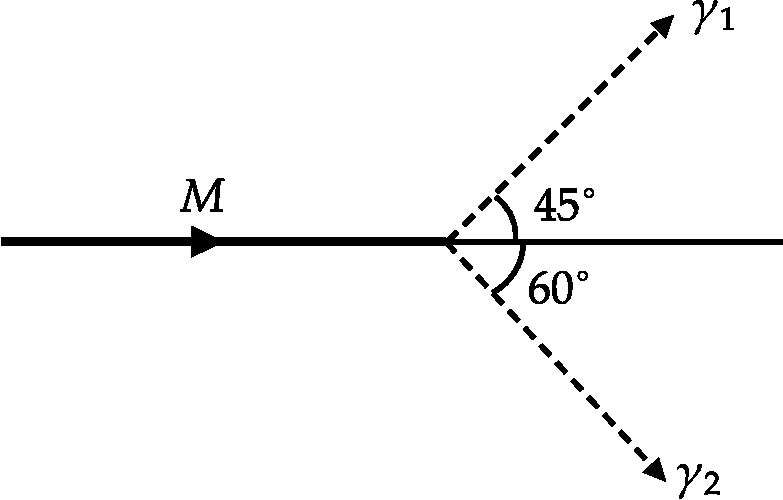
\includegraphics[height=3cm,width=5cm]{problem 17}
	\end{figure}
\begin{answer}
\begin{align*}
\sqrt{p^{2} c^{2}+M^{2} c^{4}}&=E_{1}+E_{2}=1.82 \mathrm{GeV}\\
p&=\frac{E_{1}}{c} \cos \theta_{1}+\frac{E_{2}}{c} \cos \theta_{2}=\frac{1 G e V}{c} \frac{1}{\sqrt{2}}+\frac{0.82 G e V}{c} \frac{1}{2}=\frac{1.11 G e V}{c}\\
&\Rightarrow p^{2} c^{2}+m^{2} c^{4}=3.312 \Rightarrow m^{2} c^{4}=3.312-1.23=2.08\\
&\Rightarrow m=\sqrt{2.076}=1.44
\end{align*}
\end{answer}
	\item An object travels along the $x$-direction with velocity $\frac{C}{2}$ in a frame $O$. An observer in a frame $O^{\prime}$ sees the same object travelling with velocity $\frac{C}{4}$. The relative velocity of $O^{\prime}$ with respect to $O$ in units of $c$ is.............. (up to two decimal places).
	{\exyear{GATE 2017}}
\begin{answer}
	\begin{align*}
	u_{x}^{\prime}&=\frac{C}{2}, v=\frac{C}{4}\\
	u_{x}&=\frac{u_{x}^{\prime}-v}{1-\frac{u_{x}^{\prime} v}{c^{2}}}=\frac{\frac{c}{2}-\frac{c}{4}}{1-\frac{c}{2} \cdot \frac{c}{4} \cdot \frac{1}{c^{2}}}=\frac{2 c}{7}=0.28 c
	\end{align*}
\end{answer}
	\item A spaceship is travelling with a velocity of $0.7 c$ away from a space station. The spaceship ejects a probe with a velocity $0.59$ c opposite to its own velocity. A person in the space station would see the probe moving at a speed $X_{C}$, where the value of $X$ is (up to three decimal places).
	{\exyear{GATE 2018}}
\begin{answer}$\left. \right. $\\
	\begin{minipage}{0.5\textwidth}
	\begin{align*}
	v&=0 \cdot 7 c, u_{x}^{\prime}=-0 \cdot 59 c\\
	u_{x}&=\frac{u_{x}^{\prime}+v}{1+\frac{u_{x}^{\prime} v}{c_{2}}}\\
	u_{x}&=\frac{-0.59 c+0.7 c}{1-0.7 \times 0.59}=\frac{0.11 c}{1-0.413}=\frac{0.11 c}{0.587}=0.187 c
	\end{align*}
	\end{minipage}
\begin{minipage}{0.5\textwidth}
\begin{figure}[H]
	\centering
	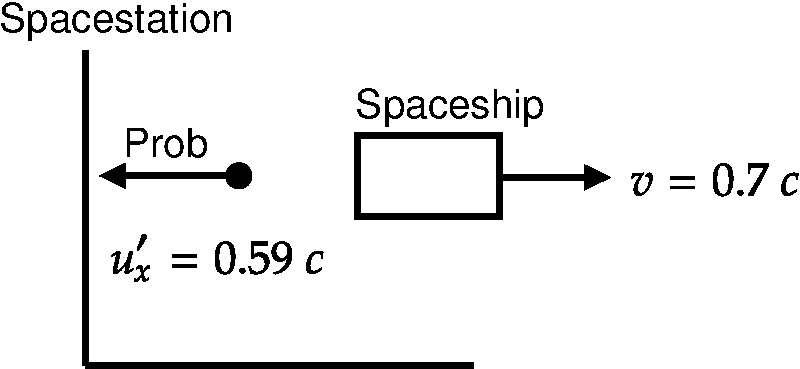
\includegraphics[height=3cm,width=5cm]{PROBLEM 18}
\end{figure}		
\end{minipage}
\end{answer}
	\item Two spaceships $A$ and $B$, each of the same rest length $L$, are moving in the same direction with speeds $\frac{4 c}{5}$ and $\frac{3 c}{5}$, respectively, where $c$ is the speed of light. As measured by $B$, the time taken by $A$ to completely overtake $B$ [see figure below] in units of $L / c$ (to the nearest integer) is
	{\exyear{GATE 2019}}$\left. \right. $\\
	\begin{minipage}{0.5\textwidth}
	\begin{figure}[H]
		\centering
		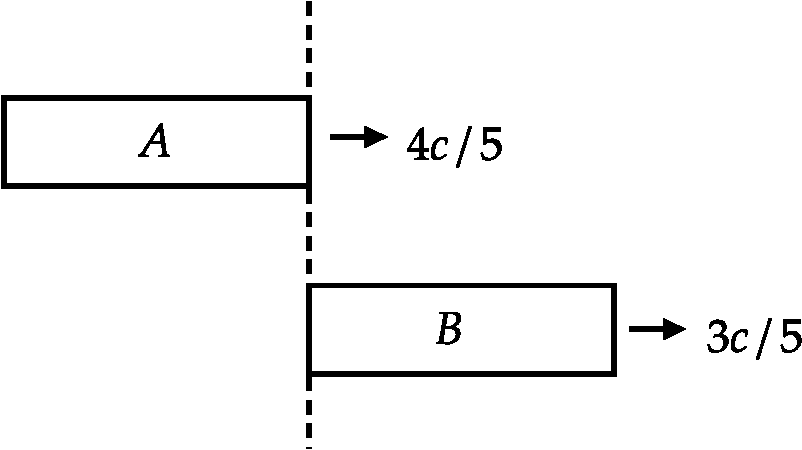
\includegraphics[height=3cm,width=5cm]{PROBLEM 19}
	\end{figure}	
	\end{minipage}
\begin{minipage}{0.5\textwidth}
	\begin{figure}[H]
		\centering
		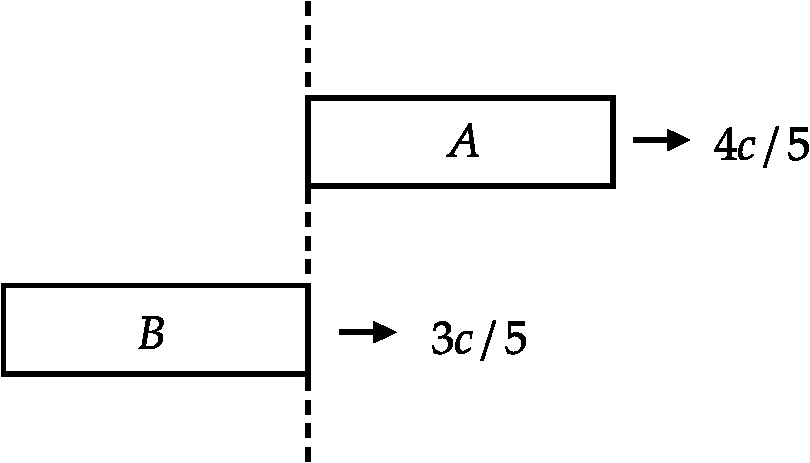
\includegraphics[height=3cm,width=5cm]{PROBLEM 20}
	\end{figure}
\end{minipage}
\begin{answer}
	\begin{align*}
	u_{A, B}&=\frac{\frac{4}{5} c-\frac{3}{5} c}{1-\frac{4}{5} c \cdot \frac{3}{5} c \cdot \frac{1}{c^{2}}}=\frac{\frac{c}{5}}{\frac{13}{25}}=\frac{5}{13} c	\\
	&\text { Kinematic equation is given by }\\
	\frac{5}{13} c \times t&=L \sqrt{1-\frac{25}{169}}+L \Rightarrow t=\frac{5 L}{c} \Rightarrow \alpha=5
	\end{align*}
\end{answer}
	\item Two events, one on the earth and the other one on the Sun, occur simultaneously in the earth's frame. The time difference between the two events as seen by an observer in a spaceship moving with velocity $0.5 c$ in the earth's frame along the line joining the earth to the Sun is $\Delta t$, where $c$ is the speed of light. Given that light travels from the Sun to the earth in $8.3$ minutes in the earth's frame, the value of $|\Delta t|$ in minutes (rounded off to two decimal places) is
	(Take the earth's frame to be inertial and neglect the relative motion between the earth and the sun)
	{\exyear{GATE 2019}}
\begin{answer}
\begin{align*}
t_{2}^{\prime}-t_{1}^{\prime}&=0 \quad x_{2}^{\prime}-x_{1}^{\prime}=8.3 \times 3 \times 10^{8} \times 60 \quad v=0.5 c\\
\Delta t&=t_{2}-t_{1}=\left(\frac{t_{2}^{\prime}+\frac{v x_{2}^{\prime}}{c^{2}}}{\sqrt{1-\frac{v^{2}}{c^{2}}}}\right)-\left(\frac{t_{1}^{\prime}+\frac{v x_{1}^{\prime}}{c^{2}}}{\sqrt{1-\frac{v^{2}}{c^{2}}}}\right)=\left(\frac{t_{2}-t_{1}^{\prime}}{\sqrt{1-\frac{v^{2}}{c^{2}}}}\right)+\frac{v}{c^{2}} \frac{\left(x_{2}^{\prime}-x_{1}^{\prime}\right)}{\sqrt{1-\frac{v^{2}}{c^{2}}}}=4.77 \min
\end{align*}	
\end{answer}
\end{enumerate}